\chapter{Convex Optimization}\label{chp:Convex Optimization}


\textit{"The great watershed in Optimization is not 
between linearity and nonlinearity, but convexity and nonconvexity. "}

%%%%%%%%%%%%ch1 section1%%%%%%%%%%%
\section{General Convex Optimization Problems}
\begin{definition}{
    (Convex Set) % 定理的名字
  }{% label
  }
    {
        a set \ $\Omega\subset \R^n$ is convex if 
         \begin{equation}
            \forall x,y \in \Omega, t\in [0,1]: x+t(y-x)\in \Omega. 
         \end{equation}


        
    }
\end{definition}

\begin{remark}
    $x+t(y-x)\in \Omega \Longleftrightarrow 
    ty + (1-t)x\in \Omega$. As $x,y$ are arbitrary points, we can say $\Omega$ is convex if
    \ $\forall x,y \in \Omega,t\in [0,1]: tx + (1-t)y\in \Omega$. 
\end{remark}

\begin{remark}
    This definition is equivalent to saying that
    all connecting lines lie inside set. 
\end{remark}

\begin{figure}[htbp]
    \begin{minipage}[t]{0.5\linewidth}
        \centering
        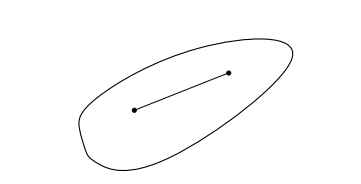
\includegraphics[width=0.8\textwidth]{figure/ch1/convex_set1.png}
        \caption{an example of a convex set}
    \end{minipage}%
    \begin{minipage}[t]{0.5\linewidth}
        \centering
        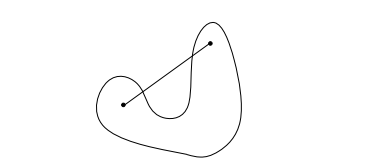
\includegraphics[width=0.8\textwidth]{figure/ch1/non_convex_set1.png}
        \caption{an example of a non convex set}
    \end{minipage}
\end{figure}


\begin{definition}{
    (Convex Function) % 定理的名字
  }{Convex Function
  }
    {
        a function $f: \Omega \rightarrow \R$ is convex, if $\Omega$ is convex and if
         \begin{equation}
            \forall x,y \in \Omega, t\in [0,1]: f(x+t(y-x))\leq f(x)+t(f(y)-f(x)). 
         \end{equation}
    }
\end{definition}
\begin{remark}
    $f(x+t(y-x))\leq f(x)+t(f(y)-f(x)) \Longleftrightarrow 
    f(ty+(1-t)x) \leq tf(y) + (1-t)f(x) $. As $x,y$ are arbitrary points, we can say $f$ is convex function if
    \ $\forall x,y \in \Omega, t\in [0,1]: f(tx+(1-t)y)\leq tf(x)+(1-t)f(y)$. 
\end{remark}
\begin{remark}
    This definition is equivalent to saying that
    all secants are above graph.
\end{remark}


\begin{figure}[htbp]
    \centering
    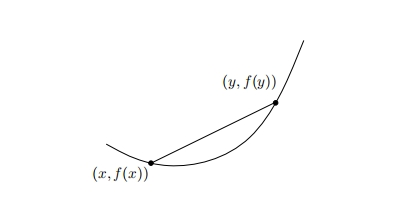
\includegraphics[width=0.6\textwidth]{figure/ch1/secant_above_graph1.png}
    \caption{For a convex function, the line segment \\ between any two points on the graph lies
    above the graph}
\end{figure}

\begin{definition}{
    (Convex Optimizaiton Problem) % 定理的名字
  }{% label
  }
    {
        an optimization problem with 
        \begin{itemize}
            \item a convex feasible set $\Omega$ and 
            \item a convex objective function $f: \Omega\rightarrow\R$
        
        \end{itemize}
        is called a "convex Optimization problem"
    }
\end{definition}






\begin{theorem}{
    (Local Implies Global Optimality for Convex Problems)
}{}
    {
        for a convex Optimization problem, every local minimum is also a global one. 
    }
\end{theorem}





\begin{proofsolution}
   
    \textcolor{LightRed}{
        Consider a local minimum $x^*$ of the convex optimization problem
        \begin{equation}
            \begin{split}
                \min_{x\in \R^n} f(x)\\
                s.t. x\in \Omega \nonumber
            \end{split}
        \end{equation}
        We will show that for each y $\in \Omega$ it holds $f(y)\geq f(x^*)$. 
    }

    Suppose that $x^*$ is not the global minmium, that is $\exists \ \widetilde{x} \in \Omega \ s.t. \ f(\widetilde{x})<f(x^*)$. \par
    Consider the line segement $x(t)=tx^*+(1-t)\widetilde{x}, t\in [0,1]$, 
        noting that $x(t)\in \Omega$ by the convexity of $\Omega$. 
        By the convexity of $f$,
        \begin{equation*}
            f(x(t))\leq tf(x^*)+(1-t)f(\widetilde{x})<tf(x^*)+(1-t)f(x^*)=f(x^*),\forall t\in [0,1]
        \end{equation*}
    \par
    As $x^*$ is a local minmium, we know that $\exists N$($N$ is a neighbourhood of $x^*$), $\forall x\in N$, $f(x)\geq f(x^*)$. 
        We can pick $t$ sufficiently to $1$ such that $x(t) \in N$. Then $f(x(t)) \geq  f(x^*)$. 
        This is a contradiction as $f(x(t)) < f(x^*)$ by the above inequality.
    \par
    Hence, $x^*$ is the global minimum. 
\end{proofsolution}

%%%%%%%%%ch1 section1 end%%%%%%%%

%%%%%%%%%ch2 section2%%%%%%%%%%%%

\section{How to Check Convexity of Functions?}

\begin{theorem}{
    (Convexity for $C^1$ Functions)
}{}
    {
        Assume that $f:\Omega\rightarrow\R$ is continuously differentiable
        and $\Omega$ is convex. Then it holds that $f$ is convex if and only if 
        \begin{equation}\label{eq:one_order_convexity_check}
            \forall x,y \in \Omega : f(y)\geq f(x) + (\nabla f(x))^T(y-x)
        \end{equation}
        $i.e.$ tangents lie below the graph. \\
    }
\end{theorem}

\begin{remark}
    The gradient (or gradient vector field) of a scalar function $f(x_1, x_2, x_3, …, x_n)$ is denoted $\nabla f$ and
    is a row vector. 
\end{remark}

\begin{figure}[htbp]
    \centering
    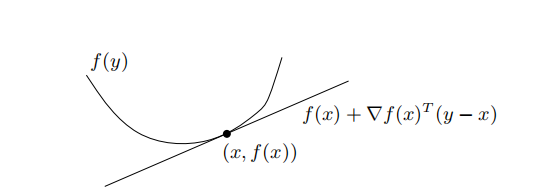
\includegraphics[width=0.6\textwidth]{figure/ch1/check_convexity1.png}
    \caption{}
\end{figure}

\begin{proofsolution}
    "$\Rightarrow$": If $f$ is convex, by definition, $\forall x\in (0,1]$, 
    \begin{equation*}
        \begin{split}
        f(x+t(y-x))\leq f(x)+t(f(y)-f(x)) \\
        \Longrightarrow f(y)-f(x)\geq \frac{f(x+t(y-x))-f(x)}{t(y-x)}\cdot (y-x)
        \end{split}
    \end{equation*}
    As $t\rightarrow 0$, we get 
    \begin{equation*}
        f(y)-f(x)\geq (\nabla f(x))^T \cdot (y-x). 
    \end{equation*}
    "$\Leftarrow$": Take any $x,y\in \Omega$ , $t\in [0,1]$  and let
    \begin{equation*}
        z = tx+(1-t)y. 
    \end{equation*}
    As $\Omega$ is convex, we have $z \in \Omega$. Then, by \eqref{eq:one_order_convexity_check}
    \begin{align*}
        f(x) & \geq f(z) + (\nabla f(z))^T(x-z)\\
        f(y) & \geq f(z) + (\nabla f(z))^T(y-z). 
    \end{align*}
    Then, 
    \begin{align*}
        tf(x) + (1-t)f(y) &\geq tf(z) + t(\nabla f(z))^T(x-z) 
        + (1-t)(f(z) + (1-t)(\nabla f(z))^T(y-z))\\
        &= f(z) + (\nabla f(z))^T(tx+(1-t)y-z)\\
        &= f(z) + (\nabla f(z))^T(z-z)\\
        &= f(tx+(1-t)y). 
    \end{align*}
    By definition\ref{def:Convex Function}, $f$ is a convex function. 
\end{proofsolution}

\begin{definition}{(Generalized inequality for Symmetric Matrices)}{}
    {
        $B$ is a symmetric matrix in $\R^{n\times n}$. Define "$B\succcurlyeq 0$" if and only if $B$ is positive semi-definite. i.e.
        \begin{align*}
            B\succcurlyeq 0 &\Longleftrightarrow \forall z \in \R^n : z^TBz\geq 0\\
                       &\Longleftrightarrow \min\{eig(B)\}\geq 0 
        \end{align*}

    }
\end{definition}

\begin{remark}
    $B\succcurlyeq 0$$\Longleftrightarrow$ all eigenvalues of $B$ are non-negative real value. $B$ is a symmetric matrix $\Rightarrow$ all eigenvalues of $B$ is real value. 
\end{remark}

% \begin{theorem}{}{}
%     A function $f:\Omega\rightarrow \R$ is convex if and only if the function $g:\R\rightarrow \R$ given by
%     $g(t)=f(x+ty)$ is convex for all $x\in \Omega$ and all $y\in \R^n$. (The domain of $g$ here is all $t$ for which $x+ty$ is in $\Omega$). 
% \end{theorem}
% \begin{proofsolution}
%     Here's a simple solution. A function $f:\R^n\rightarrow\R$
%  is convex iff the set Γf={(x1,⋯,xn,y)|f(x1,⋯,xn)≤y}⊆Rn+1
%  is convex.

% Now consider the region above the graph of g(t)
% : ΓG={(t,c)|g(t)≤c}
% . But this set is just the intersection of Γf
%  with the plane centered at x
%  generated by the vectors (v,0)
%  and (0,1)
% . Since linear subspaces are convex, Γf
%  is convex, and the intersection of two convex bodies is still convex, Γg
%  is convex and so g
%  is convex.

% The reverse direction is similar. Suppose f
%  is not convex. Then Γf
%  is not convex, and there exist points a,b∈Γf
%  such that the line between a,b
%  is not entirely contained in Γf
% . Since by definition such a line cannot be vertical, it means that the projection of such a line on to the first n
%  coordinates is again a line, and so we may choose that as the line that g
%  picks out. But then g
%  is not convex for the same reason- the line between a
%  and b
%  is not wholly contained in Γg
% .
% \end{proofsolution}

\begin{theorem}{(Convexity for $C^2$ Functions)}{two_order_convexity_check}
    {
        Assume that $f: \Omega\rightarrow \R$ is twice continuously differentiable and $\Omega$ is convex and open. 
        Then it holds that $f$ is convex if and only if for all $x\in \Omega$ the Hessian is positive semi-definite, i.e.
        \begin{equation}\label{eq:two_order_convexity_check}
            \forall x\in \Omega : \nabla^2 f(x) \succcurlyeq 0. 
        \end{equation}
    }    
\end{theorem}

\begin{proofsolution}
    Using Taylor expansion.
\end{proofsolution}


\begin{theorem}{}{}
    Consider an unconstrained optimization problem
    \begin{align*}
        \min f(x)\\
        s.t.\  x\in \R^n,
    \end{align*}
    where $f:\R^n\rightarrow \R$ is convex and differentiable. Then, 
    \begin{align*}
        \nabla f(x^*)=0 \Longleftrightarrow f(x)\geq f(x^*), \forall x\in dom(f). 
    \end{align*}
\end{theorem}

\begin{proofsolution}

\end{proofsolution}


\begin{theorem}{}{}
    Consider an optimization problem
    \begin{align*}
        \min f(x)\\
        s.t.\  x\in \Omega,
    \end{align*}
    where $f:\R^n\rightarrow \R$ is convex and differentiable and $\Omega$ is convex. Then for any $x^*\in \Omega$, 
    \begin{align*}
        \nabla f(x^*)(y-x^*)\geq 0, \forall y\in \Omega \Longleftrightarrow f(x)\geq f(x^*), \forall x\in \Omega.  
    \end{align*}
\end{theorem}

\begin{proofsolution}

\end{proofsolution}


%%%%%%%%

%%%%%%%%
